\runningheader{SAT Mathematics}{Drill Set 15}{Page \thepage\ of \numpages}

\begingradingrange{sat-drill-15}
\subsection*{SAT Drill 15}

\question[1]
Given the function $p(x)=x^4+3 x^3-2 x^2-x+b$, where $p(-1)=10$, what is the value of $b$?
\begin{choices}
  \choice $9$
  \choice $10$
  \choice $11$
  \CorrectChoice $13$
\end{choices}

\question[1]
Mr. McCoy has a class with $9^{\text{th}}$ and $10^{\text{th}}$ graders, and he asked them to share their favorite movie genre. The results are shown in the table.
\begin{center}
\vspace{0.35em}
\captionof{table}{Favorite movie genres}
\label{tab:sat-drill-15-mccoy}
\renewcommand{\arraystretch}{1.3}
\setlength{\tabcolsep}{0.5em}
\begin{adjustbox}{max width=\linewidth,clip=false,margin=0pt}
\begin{tabular}{|c|c|c|c|}
\hline
\rowcolor[HTML]{E0E0E0}
 & $9^{\text{th}}$ Grade & $10^{\text{th}}$ Grade & Total \\
\hline
Horror & 6 & 2 & 8 \\
\hline Comedy & 5 & 4 & 9 \\
\hline Action & 7 & 3 & 10 \\
\hline Total & 18 & 9 & 27 \\
\hline
\end{tabular}
\end{adjustbox}
\end{center}
Given that a randomly selected student from Mr. McCoy's class is in $9^{\text{th}}$ grade, what is the probability that they said action was their favorite movie genre?
\begin{choices}
  \choice $\dfrac{7}{27}$
  \choice $\dfrac{7}{20}$
  \CorrectChoice $\dfrac{7}{18}$
  \choice $\dfrac{7}{10}$
\end{choices}






\newpage








\question[1]
What is an integer value for $x$ that is a solution to both $12<-2 x+8$ and $4>-3 x-11$?
\begin{solution}
$-3$
\end{solution}

\question[1]
Line $g$ is defined as $-4 x+\frac{2}{3} y=5$. Line $h$ is perpendicular to line $g$. Which of the following equations could be the equation of line $h$?
\begin{choices}
  \choice $y=-\frac{1}{4} x+2$
  \CorrectChoice $y=-\frac{1}{6} x-3$
  \choice $y=\frac{3}{2} x-4$
  \choice $y=6 x+17$
\end{choices}

\question[1]
Which of the following is equivalent to the expression $\dfrac{x-2}{x+4}+\dfrac{2 x+2}{x+1}$?
\begin{choices}
  \choice $\dfrac{x}{x+4}$
  \choice $\dfrac{3 x}{2 x+5}$
  \CorrectChoice $\dfrac{3(x+2)}{x+4}$
  \choice $\dfrac{3(x+2)}{x+1}$
\end{choices}







\newpage







\question[1]
What value of $d$ is the solution in the given equation?
\[
  4=\frac{32}{3 d-7}
\]
\begin{solution}
$5$
\end{solution}

\question[1]
The scatterplot shows data on 15 libraries and includes a line of best fit. For the library that spent the smallest percentage of its budget on technology, which of the following is closest to the difference between the actual percentage and the percentage predicted by the line of best fit?
\begin{center}
  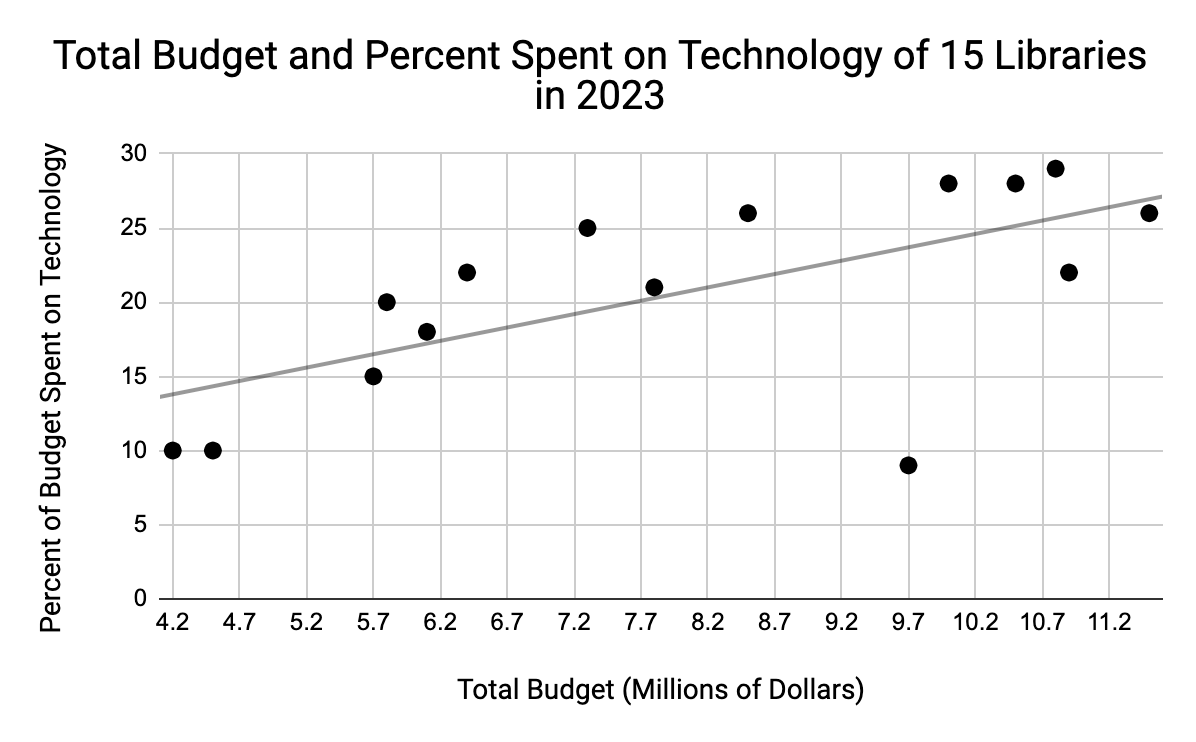
\includegraphics[width=0.90\linewidth]{images/cus52}
\end{center}
\begin{choices}
  \choice $4\%$
  \CorrectChoice $9\%$
  \choice $15\%$
  \choice $24\%$
\end{choices}

\question[1]
Which of the following expressions is equivalent to $\left(\sin 33^{\circ}\right)\left(\cos 57^{\circ}\right)-\left(\cos 33^{\circ}\right)\left(\sin 57^{\circ}\right)$?
\begin{choices}
  \choice $2\left(\sin 33^{\circ}\right)\left(\cos 57^{\circ}\right)$
  \CorrectChoice $\left(\sin 33^{\circ}\right)^2-\left(\sin 57^{\circ}\right)^2$
  \choice $\left(\sin 33^{\circ}\right)^2-\left(\cos 57^{\circ}\right)^2$
  \choice $2\left(\sin 33^{\circ}\right)-2\left(\cos 33^{\circ}\right)$
\end{choices}





\newpage




\question[1]
In the figure, $\overline{M R}, \overline{N Q}$, and $\overline{O P}$ are parallel. Points $N$ and $Q$ lie on $\overline{M O}$ and $\overline{P R}$, respectively. If $M N=10.6$, $N O=8$, and $P Q=6.4$, what is the length of $\overline{P R}$?
\begin{center}
  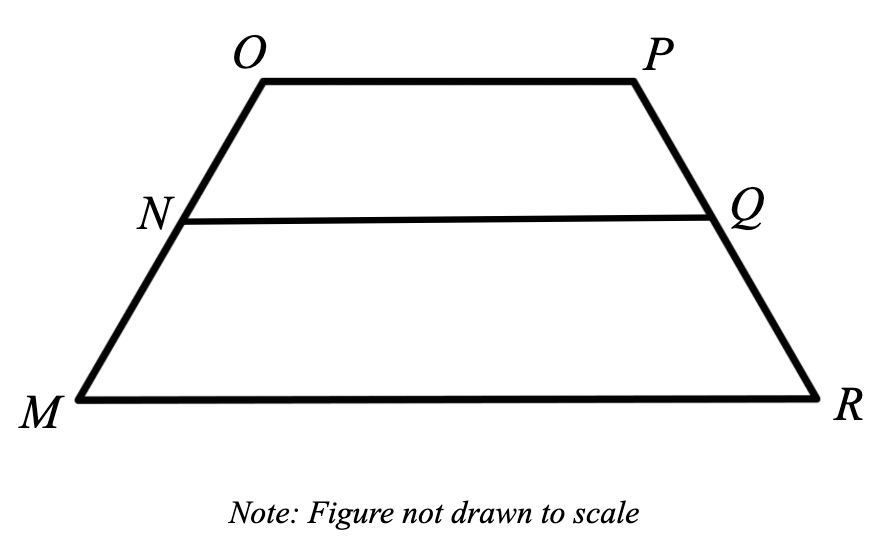
\includegraphics[width=0.90\linewidth]{images/cus53}
\end{center}
\begin{choices}
  \choice $4.83$
  \choice $8.48$
  \CorrectChoice $11.23$
  \choice $14.88$
\end{choices}

\question[1]
The middle school math teachers in the Hayview School District wanted to know if using a calculator on math tests helped improve test scores. All middle school math students in the district took the same test, and a random sample was selected to be allowed to use a calculator. It was determined that those who used a calculator scored higher on the test compared to students who did not use a calculator. Which of the following conclusions can be drawn?
\begin{choices}
  \choice Any student who uses a calculator will typically score higher on math tests.
  \choice Middle school students in the Hayview school district perform better on a math test when allowed to use a calculator.
  \choice Teachers should allow the use of calculators when teaching math to improve test scores.
  \CorrectChoice No conclusion can be drawn concerning calculator use and test scores.
\end{choices}






\newpage





\question[1]
The expression $10 x^2+n x-72$, in which $n$ is a constant, is equivalent to $(p x+4 j)(q x-k)$, in which $p, q, j$, and $k$ are integer constants. Which of the following must be an integer?
\begin{choices}
  \CorrectChoice $\dfrac{18}{k}$
  \choice $\dfrac{4}{n}$
  \choice $\dfrac{10}{j}$
  \choice $\dfrac{72}{q}$
\end{choices}


\question[1]
Noa and Lilliana have a cake business. For each cake, they spend $\$37.50$ on ingredients, and they sell each cake for $\$65$. They pay their friend Francesca $15\%$ of their profit to do marketing, and they split the remaining profit evenly. If Noa makes $\$5,420$ in a particular month, which of the following equations can be used to find how many cakes, $x$, the business sold in that month?
\begin{choices}
  \choice $\dfrac{(0.15)(65-37.5)x}{2}=5,420$
  \CorrectChoice $\dfrac{(0.85)(65-37.5)x}{2}=5,420$
  \choice $2((0.15)(65-37.5)x)=5,420$
  \choice $2((0.85)(65-37.5)x)=5,420$
\end{choices}


\question[1]
If $\dfrac{9 m}{2 n}=\dfrac{1}{4}$, what is the value of $\dfrac{18 n}{m}$?
\begin{solution}
324
\end{solution}






\newpage




\question[1]
The functions $f$ and $g$ are defined as $f(x)=-\dfrac{4}{5} x-13$ and $g(x)=\dfrac{3}{10} x+7$. The function $h(x)$ is defined as $f(g(x))$. What is the $x$-coordinate of the $x$-intercept of $h(x)$?
\begin{choices}
  \CorrectChoice $-\dfrac{155}{2}$
  \choice $-\dfrac{475}{12}$
  \choice $\dfrac{155}{12}$
  \choice $\dfrac{2,275}{6}$
\end{choices}


\question[1]
A positive integer $a$ is $4.5\%$ greater than a positive integer $b$, a positive integer $c$ is $2.7\%$ less than $b$, and a positive integer $d$ is $7.8\%$ of $c$. Approximately how many times greater is $a$ than $d$?
\begin{choices}
  \choice $0.07$
  \choice $0.96$
  \choice $12.82$
  \CorrectChoice $13.77$
\end{choices}

\question[1]
\[
  \begin{gathered}
  \frac{p}{2} x-\frac{q}{7} y=9 \\
  p x-q y=10
  \end{gathered}
\]
In the system of equations above, $p$ and $q$ are constants, and the system has one solution. What is the solution to the system?
\begin{choices}
  \choice $\left(\dfrac{146}{9p},\, \dfrac{56}{9q}\right)$
  \choice $\left(-\dfrac{6}{5p},\, -\dfrac{56}{5q}\right)$
  \choice $\left(\dfrac{56}{5q},\, \dfrac{106}{5p}\right)$
  \CorrectChoice $\left(\dfrac{106}{5p},\, \dfrac{56}{5q}\right)$
\end{choices}







\newpage




\question[1]
A line with the equation $y = m x + 9$ intersects the parabola with the equation $y = x^2 - 4x + 10$ at exactly one point. What is the sum of the possible values for $m$?
\begin{solution}
-8
\end{solution}

\question[1]
The figure shows a cylindrical fish tank that is completely filled with water. If the water is poured into a cube with a side length equal to the diameter of the tank, what will the height of the water be?
\begin{center}
  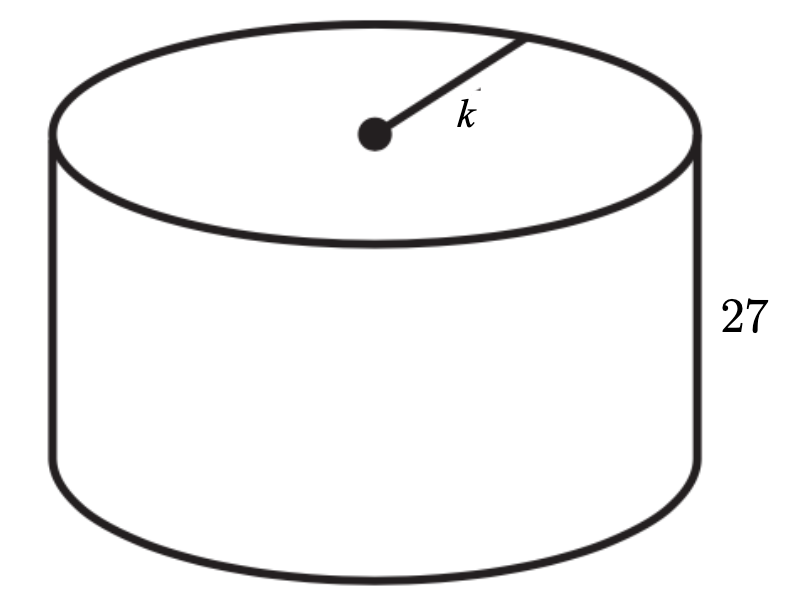
\includegraphics[width=0.65\linewidth]{images/cus54}
\end{center}
\begin{choices}
  \choice $27$
  \choice $27\pi$
  \choice $\dfrac{27\pi}{4}$
  \choice $\dfrac{27\pi}{8k}$
\end{choices}

\question[1]
The equation $y=\sqrt{2 x+7}$ intersects a line with the equation $y=\frac{1}{4} x+b$ at its $x$-intercept and one other point. What is the $x$-coordinate of the other point of intersection?
\begin{choices}
  \choice $-\dfrac{7}{2}$
  \choice $\dfrac{7}{8}$
  \choice $8$
  \CorrectChoice $\dfrac{57}{2}$
\end{choices}






\newpage




\question[1]
\[
  f(x)=(x-a)(x-b)
\]
The function $f$ is defined by the above equation. The function $g$ is defined by $g(x)=f(x+5)$, and the vertex of $g(x)$ can be found at the point $\left(-\dfrac{7}{4}, \dfrac{9}{4}\right)$. What is the value of $a+b$?
\begin{solution}
$\frac{13}{2}$
\end{solution}

\question[1]
In the figure, the circles $O$ and $P$ are congruent. The length of $\overline{O P}$ is $x$, and $\overline{A C}$ is half the radius of the circle $O$. Which of the following expressions represents the area of sector $A P D$?
\begin{center}
  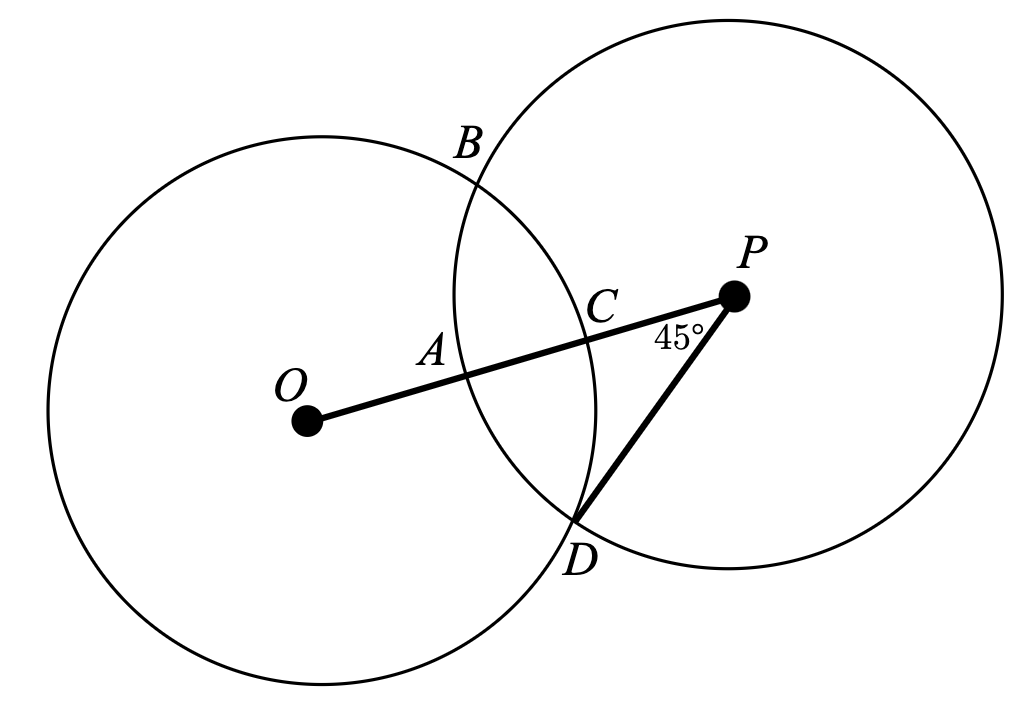
\includegraphics[width=0.90\linewidth]{images/cus55}
\end{center}
\begin{choices}
  \choice $\dfrac{1}{6} \pi x$
  \choice $\dfrac{4}{9} \pi x^2$
  \choice $\dfrac{1}{12} \pi x^2$
  \choice $\dfrac{1}{18} \pi x^2$
\end{choices}






\newpage




\question[1]
\[
  x^2+a x+b=0
\]
In the given equation, $a$ and $b$ are positive integer constants. If the equation has one distinct integer solution, what is the value of $a$?
\begin{choices}
  \choice $b$
  \choice $\sqrt{2} b$
  \CorrectChoice $2 \sqrt{b}$
  \choice $2 b$
\end{choices}

\question[1]
What value of $p$ would make the equation $2.5 p x + p = 7.5 x - 10$ have no solution?
\begin{choices}
  \choice $-10$
  \choice $-3$
  \CorrectChoice $3$
  \choice $\dfrac{10}{3}$
\end{choices}

\question[1]
At how many unique values of $x$ does $g(x) = 0$ for the polynomial function $g(x) = (x-2)^2(x+3)^3(x-5)$?
\begin{choices}
  \choice $2$
  \CorrectChoice $3$
  \choice $4$
  \choice $6$
\end{choices}






\newpage




\question[1]
AJ purchased $4$ packs of batteries. He added them to the $8$ batteries he had at home. After giving half to his brother, he now has $32$ batteries left. How many batteries are in $2$ packs of batteries?
\begin{choices}
  \choice $2$
  \choice $4$
  \choice $14$
  \CorrectChoice $28$
\end{choices}

\question[1]
\[
k x + 4 y = 12
\]
The equation above is the equation of line $p$, where $k$ is a constant. The equation has an $x$-intercept of $4$. What is the value of $k$?
\begin{solution}
3
\end{solution}






\newpage




\question[1]
In which of the following tables is the relationship between $x$ and the corresponding values of $y$ exponential?
\medskip
\noindent (A)
\begin{center}
  \renewcommand{\arraystretch}{1.3}
  \setlength{\tabcolsep}{0.5em}
  \begin{tabular}{|l|l|l|l|l|}
  \hline
  \rowcolor[HTML]{E0E0E0}
  $x$ & 0 & 1 & 2 & 3 \\
  \hline
  $y$ & 4 & 8 & 12 & 16 \\
  \hline
  \end{tabular}
\end{center}

\noindent (B)
\begin{center}
  \renewcommand{\arraystretch}{1.3}
  \setlength{\tabcolsep}{0.5em}
  \begin{tabular}{|l|l|l|l|l|}
  \hline
  \rowcolor[HTML]{E0E0E0}
  $x$ & 0 & 1 & 2 & 3 \\
  \hline
  $y$ & 4 & 5 & 8 & 13 \\
  \hline
  \end{tabular}
\end{center}

\noindent (C)
\begin{center}
  \renewcommand{\arraystretch}{1.3}
  \setlength{\tabcolsep}{0.5em}
  \begin{tabular}{|l|l|l|l|l|}
  \hline
  \rowcolor[HTML]{E0E0E0}
  $x$ & 0 & 1 & 2 & 3 \\
  \hline
  $y$ & 4 & 2 & 1 & $\tfrac{1}{2}$ \\
  \hline
  \end{tabular}
\end{center}

\noindent (D)
\begin{center}
  \renewcommand{\arraystretch}{1.3}
  \setlength{\tabcolsep}{0.5em}
  \begin{tabular}{|l|l|l|l|l|}
  \hline
  \rowcolor[HTML]{E0E0E0}
  $x$ & 0 & 1 & 2 & 3 \\
  \hline
  $y$ & 4 & $2\tfrac{1}{2}$ & 1 & $-\tfrac{1}{2}$ \\
  \hline
  \end{tabular}
\end{center}

\begin{choices}
  \choice (A)
  \choice (B)
  \CorrectChoice (C)
  \choice (D)
\end{choices}






\newpage




\question[1]
A semicircle is attached to a square, as shown.
\begin{center}
  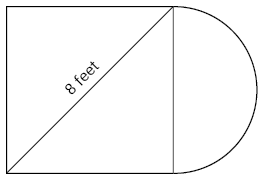
\includegraphics[width=0.90\linewidth]{images/cus56}
\end{center}
What is the area of the given figure, in square feet?
\begin{choices}
  \choice $32 + 4\pi$
  \CorrectChoice $32 + 8\pi$
  \choice $32 + 16\pi$
  \choice $32 + 32\pi$
\end{choices}

\question[1]
A statistically significant sample of 200 biology teachers were selected at random from high schools in Texas. The teachers were asked if they include lab activities in their classrooms or not, and 127 of the teachers said they do include lab activities in their classrooms. Which of the following is the largest population to which the results of the survey can be applied?
\begin{choices}
  \choice The 200 biology teachers surveyed
  \CorrectChoice All high school biology teachers in Texas
  \choice All high school science teachers in Texas
  \choice All high school biology teachers in the United States
\end{choices}






\newpage




\question[1]
Which of the following expressions is equivalent to $\sqrt[9]{k^7}$, such that $k>0$?
\begin{choices}
  \choice $\dfrac{9}{7}k$
  \choice $k^{\frac{21}{36}}$
  \CorrectChoice $k^{\frac{49}{63}}$
  \choice $k^{\frac{18}{14}}$
\end{choices}

\question[1]
The students at Western Middle School were all asked to share if they were left-handed, right-handed, or ambidextrous. The results are shown in the table.
\begin{center}
\vspace{0.35em}
\captionof{table}{Handedness by Grade}
\label{tab:sat-drill-15-handedness}
\renewcommand{\arraystretch}{1.3}
\setlength{\tabcolsep}{0.5em}
\begin{adjustbox}{max width=\linewidth,clip=false,margin=0pt}
\begin{tabular}{|c|c|c|c|}
\hline
\rowcolor[HTML]{E0E0E0}
& Left-handed & Right-handed & Ambidextrous \\
\hline Sixth Grade & 21 & 156 & 5 \\
\hline Seventh Grade & 29 & 185 & 3 \\
\hline Eighth Grade & 22 & 178 & 7 \\
\hline
\end{tabular}
\end{adjustbox}
\end{center}
Given that a randomly selected student is in sixth grade, what is the probability that the student is left-handed?
\begin{solution}
$\frac{3}{26}$
\end{solution}






\newpage




\question[1]
\[
A(j)=\frac{3}{4}(j-75.4)+15
\]
In a certain role-playing game, wizards must transform real-world physical energy, measured in joules $(j)$, into magical energy, measured in arcana units $(A)$, to perform their spells. The function above shows the relationship between $A$ and $j$. If a teleportation spell requires $1{,}097.4$ more joules to cast than a transfiguration spell, how many more arcana units would the teleportation spell require than the transfiguration spell?
\begin{solution}
$823.05$
\end{solution}

\question[1]
To create data set $B$, each value in data set $A$ is tripled and then decreased by $7$. If the mean of data set $B$ is $x$, what is the mean of data set $A$ in terms of $x$?
\begin{choices}
  \choice $3x-7$
  \choice $3(x-7)$
  \choice $\dfrac{1}{3}x+7$
  \CorrectChoice $\dfrac{1}{3}(x+7)$
\end{choices}






\newpage




\question[1]
A bakery uses flour and sugar in a ratio of $5:2$ to make its signature cake batter. A customer places a special order requesting 3 chocolate cakes that are more moist. To make the cake more moist, the head baker decides to increase the amount of sugar per cake by $20\%$ and not change the amount of flour. However, due to miscommunication, the bakery used the regular batter ratio for the first cake and the modified batter ratio for the remaining two cakes. What is the overall flour to sugar ratio used across all three cakes?
\begin{choices}
  \choice $15:6$
  \choice $15:7$
  \CorrectChoice $75:34$
  \choice $75:36$
\end{choices}

\question[1]
\[
\begin{gathered}
7x-8y = 17y - q \\
p\,y = 3 - 4x
\end{gathered}
\]
In the given system of equations, $p$ and $q$ are constants. If the system has infinitely many solutions, what is the value of $q$?
\begin{choices}
  \choice $-\dfrac{100}{7}$
  \CorrectChoice $-\dfrac{21}{4}$
  \choice $-3$
  \choice $-\dfrac{21}{100}$
\end{choices}






\newpage




\question[1]
\[
y=\frac{4}{x^2-7x+c}
\]
If the expression above is undefined at two different values of $x$ and $c$ is an integer, what is the largest possible value of $c$?
\begin{solution}
12
\end{solution}


\question[1]
\[
\frac{x^2}{\sqrt{9x^2+a^2}} \;=\; 87 \;-\; \frac{a^2}{9\sqrt{9x^2+a^2}}
\]
In the equation above, $a$ is a constant. Which of the following is a solution to the equation?
\begin{choices}
  \choice $261-\dfrac{a}{3}$
  \choice $\sqrt{783-\dfrac{a^2}{9}}$
  \CorrectChoice $\sqrt{68{,}121-\dfrac{a^2}{9}}$
  \choice $\sqrt{613{,}089-\dfrac{a^2}{9}}$
\end{choices}

\question[1]
\[
\begin{gathered}
y = a x^2 - 72x + c \\
y = x^2 - b x + 18
\end{gathered}
\]
In the system of equations above, $a,b,c$ are integer constants, and the two equations have the same $x$-intercepts. If the $x$-intercepts are integer values, what is the value of $c$?
\begin{solution}
144
\end{solution}






\newpage




\question[1]
If $15\%$ of $ab$ is $c$, what is $20\%$ of $(0.5a)(0.75b)$?
\begin{choices}
  \choice $0.01875\,c$
  \choice $0.075\,c$
  \choice $0.375\,c$
  \CorrectChoice $0.5\,c$
\end{choices}

\question[1]
Circle $A$ in the $xy$-plane has center at $(3,-4)$ and a diameter of $7$. Circle $B$ is created by translating Circle $A$ 4 units to the right and 2 units down and tripling the diameter. An equation for circle $B$ is
\[
x^2+y^2+p x+q y+r=0.
\]
What is the value of $p+q+r$?
\begin{choices}
  \choice $-358$
  \CorrectChoice $-27.25$
  \choice $-12.5$
  \choice $51.25$
\end{choices}

\question[1]
Cube $B$ has a volume of $804{,}357$ cubic feet. The ratio of a side length of Cube $B$ to a side length of Cube $A$ is $3:1$. What is the surface area, in square feet, of Cube $A$?
\begin{choices}
  \CorrectChoice $5{,}766$
  \choice $24{,}948$
  \choice $29{,}791$
  \choice $467{,}046$
\end{choices}






\newpage




\question[1]
The function $f(x)$ is a quadratic function. The maximum value of the function is at $f(p)=q$, where $p$ and $q$ are positive real numbers. The graph of $f(x)$ intersects the $x$-axis at the point $(-4,0)$. What must be the coordinates of the other $x$-intercept of the function?
\begin{choices}
  \choice $(4,0)$
  \choice $(p+4,0)$
  \CorrectChoice $(2p+4,0)$
  \choice $(-2p+4,0)$
\end{choices}

\question[1]
In the diagram, $\overline{BG}$ bisects $\angle FBD$, $\overline{DE}$ bisects $\angle FDB$, and $\overline{FD}\cong\overline{BD}$. What is the value of $x$?
\begin{center}
  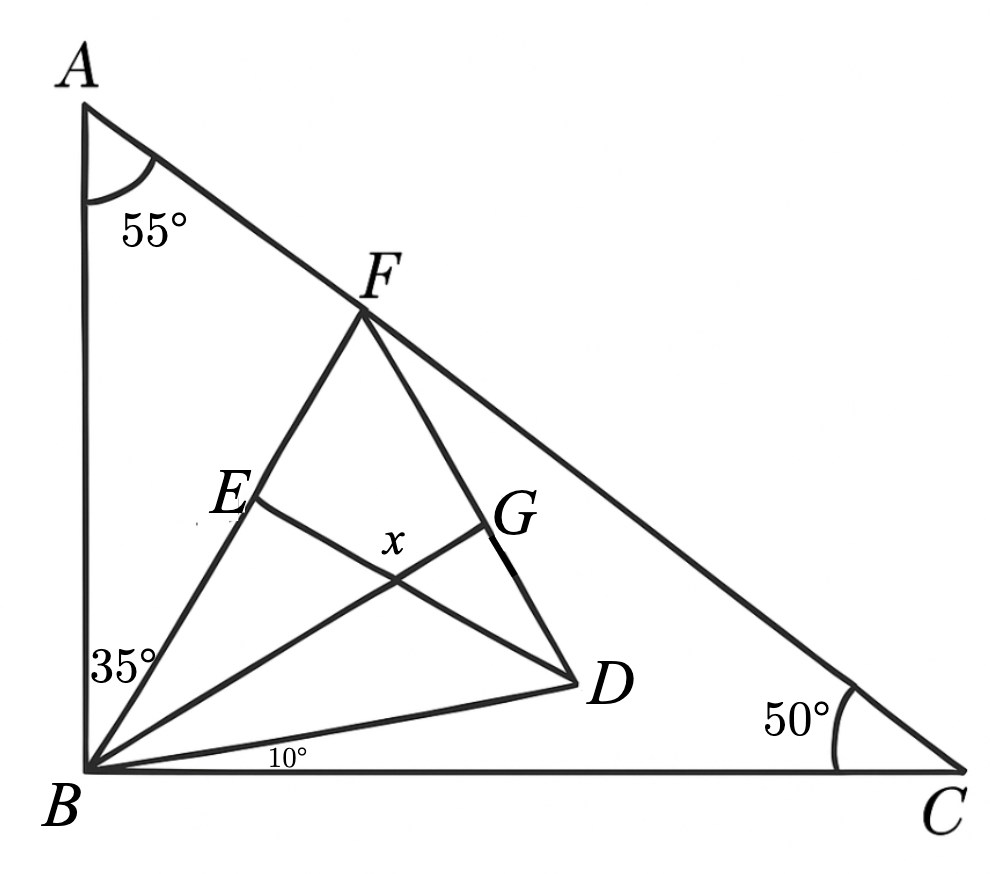
\includegraphics[width=0.90\linewidth]{images/cus57}
\end{center}
\begin{solutionorbox}
\end{solutionorbox}






\newpage




\question[1]
If \(\dfrac{\sqrt[3]{x^7}}{\sqrt[2]{x^3}}=x^a\) and \(\dfrac{\sqrt[4]{y^5}}{\sqrt[3]{y^8}}=y^b\), what is the value of \(a-b\)?
\begin{choices}
  \choice $-\dfrac{17}{12}$
  \choice $-\dfrac{7}{12}$
  \choice $\dfrac{5}{6}$
  \CorrectChoice $\dfrac{9}{4}$
\end{choices}

\endgradingrange{sat-drill-15}
